\chapter{Прогнозування за моделлю залежності}

Маємо набір випадкових процесів $X_i, i=1..6$,
що не містять аномальних точок,
проте містять помилки.
Потрібно побудувати їх прогноз,
модель залежності $Y$ від цих процесів,
та на основі цього створити прогноз для $Y$.

Зобразимо дані процеси графічно на рис. \ref{fig:x:source}.
\begin{figure}[h!]
  \centering
  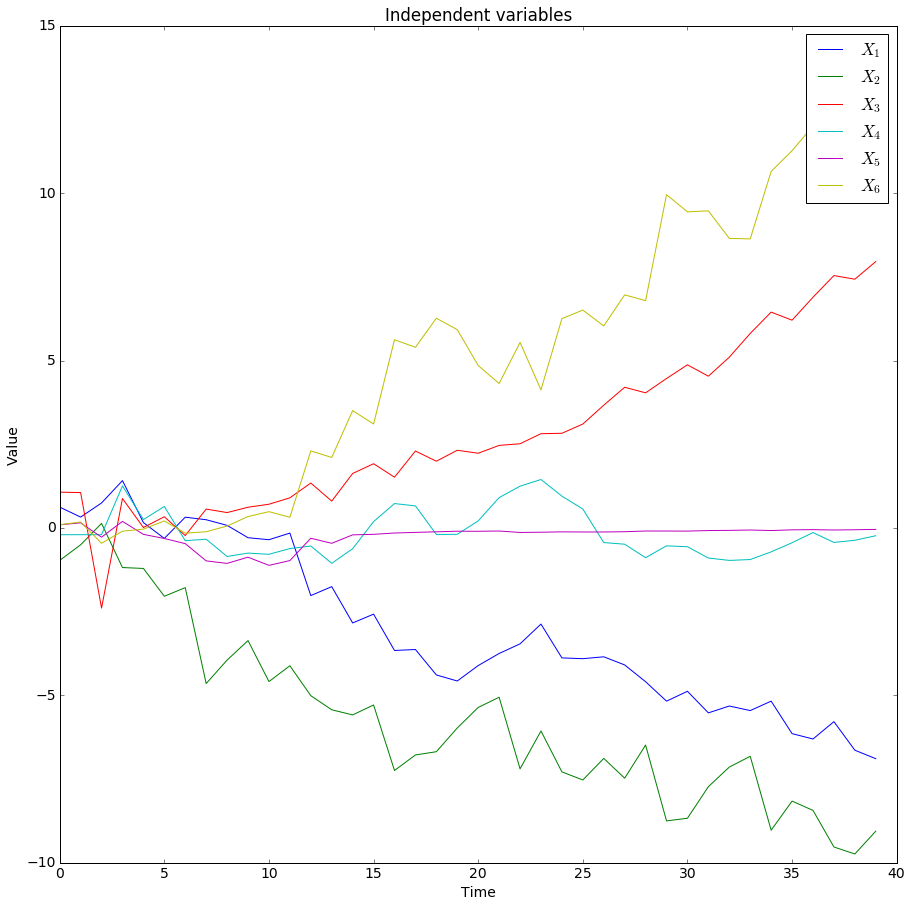
\includegraphics[width=\textwidth]{Coursework2_files/Coursework2_6_0.png}
  \caption{Графіки процесів $X$}
  \label{fig:x:source}
\end{figure}
% \begin{center}
% \adjustimage{max size={0.9\linewidth}{0.9\paperheight}}{Coursework2_files/Coursework2_6_0.png}
% \end{center}

\section{Зглажування}

В даному розділі не будемо детально зупинятися на тому,
что вже було розглянуто при аналізі $Y$.

Лінії тренду для всіх $X$ знайдені за допомогою
експоненційно зваженого ковзкого середнього (рис. \ref{fig:x:trends}).
\begin{figure}[h!]
  \centering
  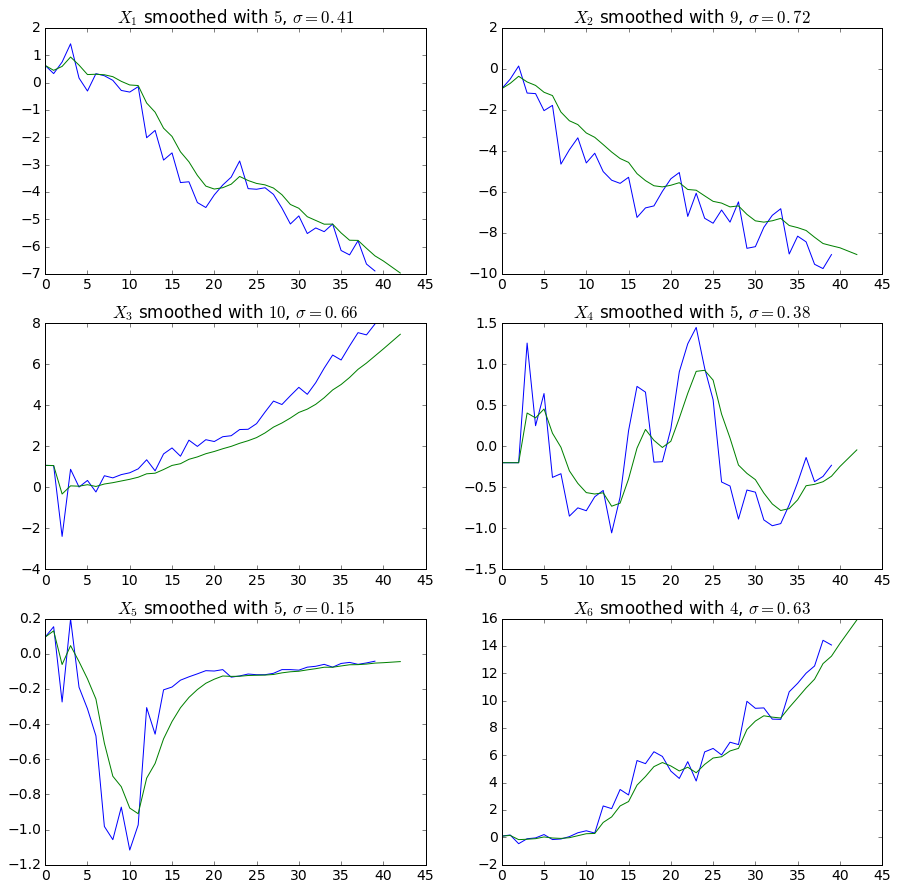
\includegraphics[width=\textwidth]{Coursework2_files/Coursework2_7_0.png}
  \caption{Графіки процесів $X$ та їх трендів}
  \label{fig:x:trends}
\end{figure}
% \begin{center}
% \adjustimage{max size={0.9\linewidth}{0.9\paperheight}}{Coursework2_files/Coursework2_7_0.png}
% \end{center}

Графіки автокореляцій показали,
що достатньо обрати два минулі члені послідовності,
щоб зробити прогноз для наступного.
Щоправда, $X_3$ має дуже багато залежностей,
це може означати,
що кожне наступне значення залежить від попереднього
і ми маємо Марковський ланцюг (рис. \ref{fig:x:autocorrelation}).
\begin{figure}[h!]
  \centering
  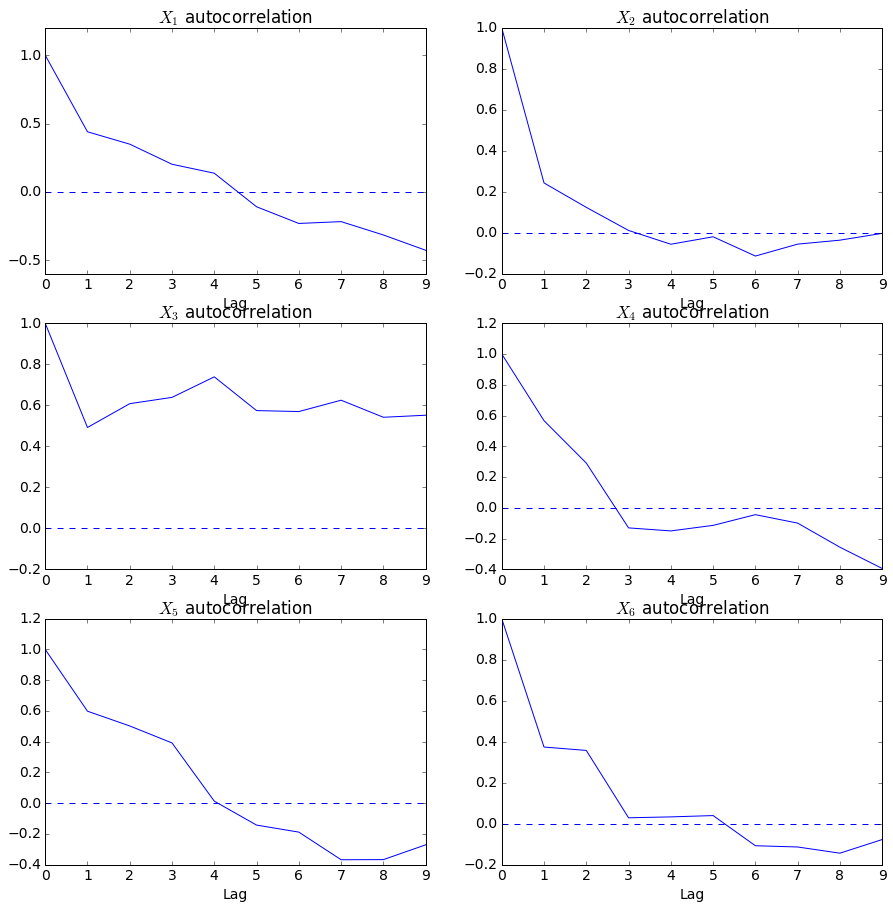
\includegraphics[width=\textwidth]{Coursework2_files/Coursework2_8_0.png}
  \caption{Графіки автокореляцій процесів $X$ за різних лагів $\tau$}
  \label{fig:x:autocorrelation}
\end{figure}
% \begin{center}
% \adjustimage{max size={0.9\linewidth}{0.9\paperheight}}{Coursework2_files/Coursework2_8_0.png}
% \end{center}

Фильтр, що враховує невипадкові помилки,
дуже добре відповідає дійсним даним (рис. \ref{fig:x:trends:errors}.
\begin{figure}[h!]
  \centering
  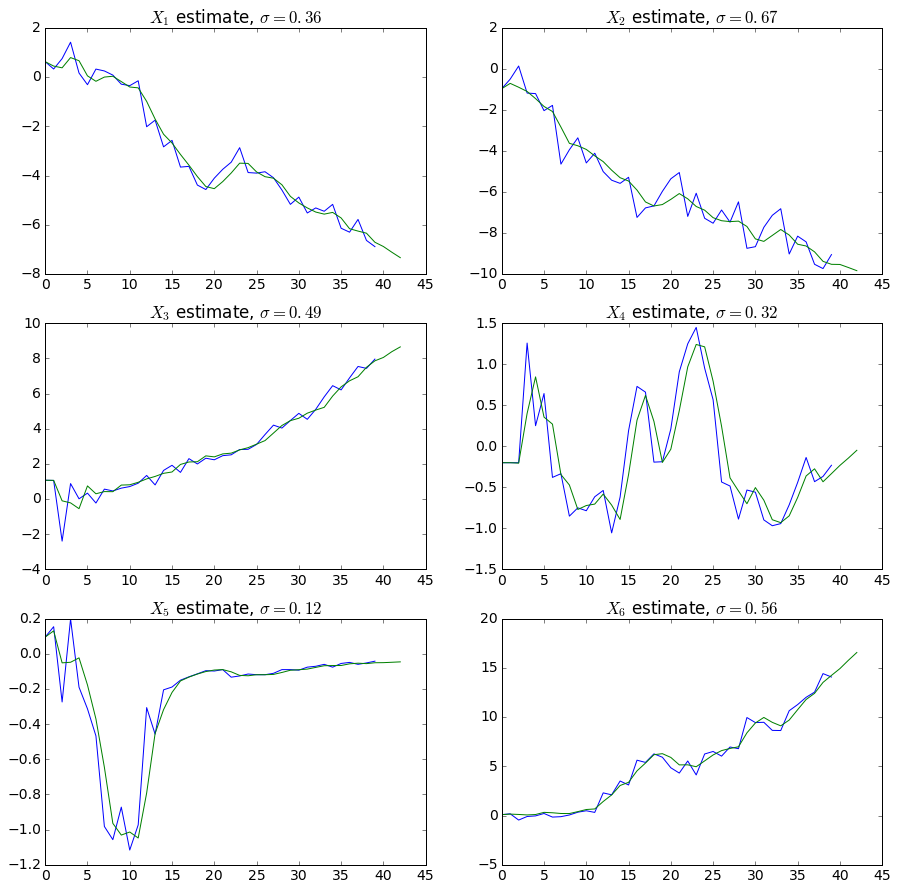
\includegraphics[width=\textwidth]{Coursework2_files/Coursework2_9_0.png}
  \caption{Оцінки $X$ з урахуванням невипадкових помилок}
  \label{fig:x:trends:errors}
\end{figure}
% \begin{center}
% \adjustimage{max size={0.9\linewidth}{0.9\paperheight}}{Coursework2_files/Coursework2_9_0.png}
% \end{center}

\section{Прогноз часових рядів}

\begin{figure}[h!]
  \centering
  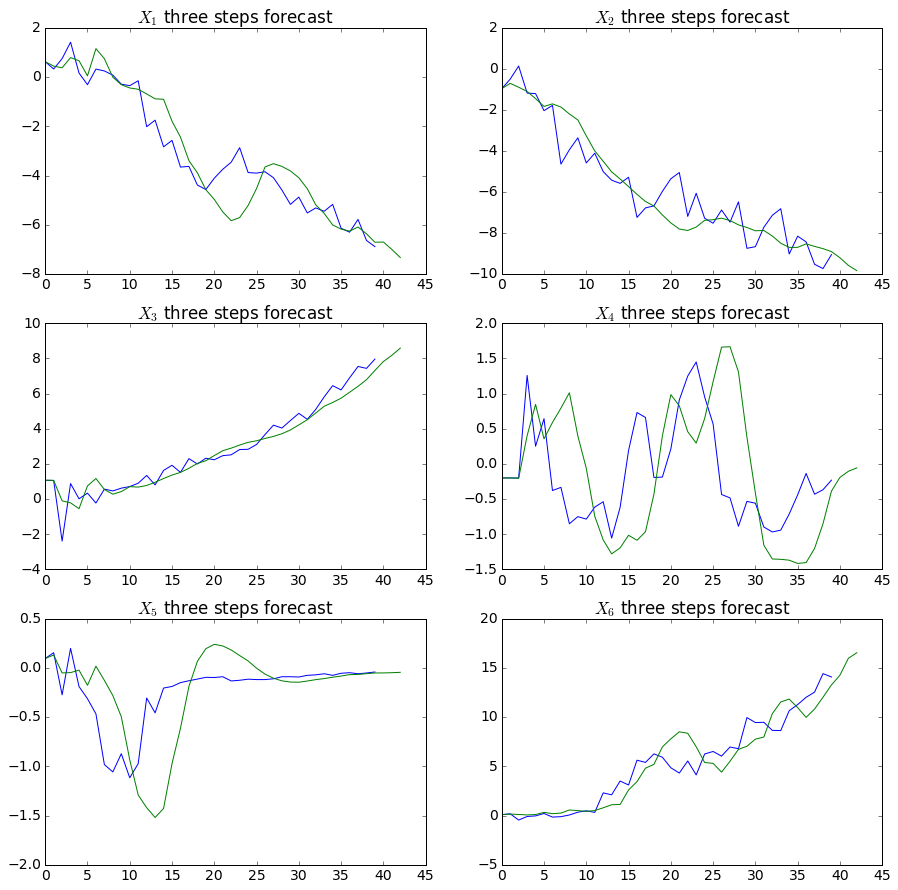
\includegraphics[width=\textwidth]{Coursework2_files/Coursework2_14_0.png}
  \caption{Прогнози $X$}
  % \label{fig:x:trends:errors}
\end{figure}
% \begin{center}
% \adjustimage{max size={0.9\linewidth}{0.9\paperheight}}{Coursework2_files/Coursework2_14_0.png}
% \end{center}

\section{Побудова моделі}

Для того, щоб знайти залежність між $Y$ та $X$,
було використано не тільки $X_i$,
але і їх попарні поелементні добутки $X_i \cdot X_j$.
Ці значення називаємо регресорами.

Ітеративний метод побудови моделі полягає в наступному:
\begin{enumerate}
  \item першим регресором є ряд, що складається з одиниць
    (очевидно, що перший коефіцієнт --- середнє значення $Y$);
  \item з невикористаних регресорів обирається той,
    що найбільше корелює з залишками ---
    різницею між вхідними даними $Y$ та поточною моделлю $\tilde{Y}$;
  \item методом найменших квадратів перераховуються коефіцієнти,
    що множаться на обрані регресори;
  \item за допомогою $F$-тесту перевіряється,
    чи дав цей новий регресор значний приріст якості;
  \item якщо якість зросла і залишилися ще невикористані регресори,
    обираємо наступний регресор;
  \item якщо ні, маємо модель.
\end{enumerate}

Було отримано модель з регресорами $\mathcal{1}$,
$X_2 \cdot X_6$, $X_3 \cdot X_5$, $X_4 \cdot X_5$
та коефіцієнтами $-3.33$, $1.75$, $15.6$, $22.67$.
Маємо графік з вхідним рядом $Y$
та його прогнозом, що було побудовано на основі прогнозів $X$
(рис. \ref{fig:y:forecast:x}).

\begin{figure}[h!]
  \centering
  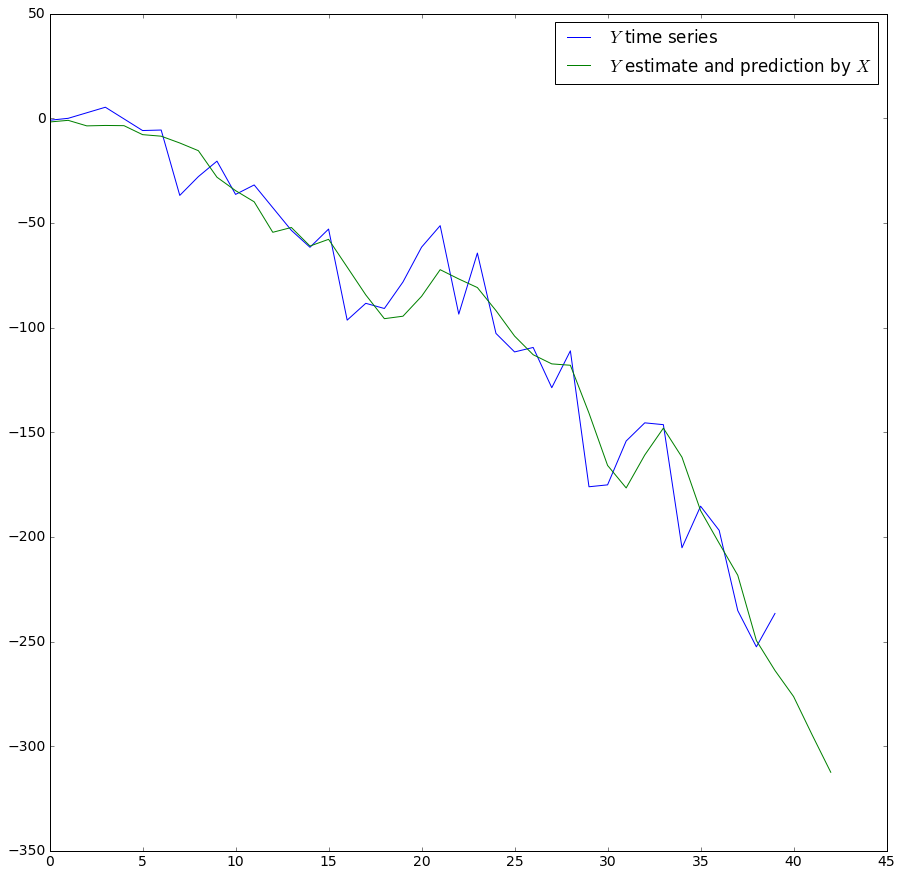
\includegraphics[width=\textwidth]{Coursework2_files/Coursework2_13_0.png}
  \caption{Прогнози $Y$ як моделі $X$}
  \label{fig:y:forecast:x}
\end{figure}
% \begin{center}
% \adjustimage{max size={0.9\linewidth}{0.9\paperheight}}{Coursework2_files/Coursework2_13_0.png}
% \end{center}
